%%%%%%%%%%%%%%%%%%%%%%%%%%%%%%%%%%%%%%%%%
% Thin Sectioned Essay
% LaTeX Template
% Version 1.0 (3/8/13)
%
% This template has been downloaded from:
% http://www.LaTeXTemplates.com
%
% Original Author:
% Nicolas Diaz (nsdiaz@uc.cl) with extensive modifications by:
% Vel (vel@latextemplates.com)
%
% License:
% CC BY-NC-SA 3.0 (http://creativecommons.org/licenses/by-nc-sa/3.0/)
%
%%%%%%%%%%%%%%%%%%%%%%%%%%%%%%%%%%%%%%%%%

%----------------------------------------------------------------------------------------
%	PACKAGES AND OTHER DOCUMENT CONFIGURATIONS
%----------------------------------------------------------------------------------------

\documentclass[a4paper, 12pt]{article} % Font size (can be 10pt, 11pt or 12pt) and paper size (remove a4paper for US letter paper)

\usepackage[protrusion=true,expansion=true]{microtype} % Better typography
\usepackage{graphicx} % Required for including pictures
\usepackage[utf8]{inputenc}
\usepackage[margin=1.0in]{geometry}
\usepackage{url}
\usepackage{fancyhdr}
\usepackage{amsmath}
\usepackage{setspace}
\usepackage{enumitem}
\usepackage{float}
\setlength\parindent{0pt} % Removes all indentation from paragraphs

\usepackage[T1]{fontenc} % Required for accented characters
\usepackage{times} % Use the Palatino font

\usepackage{listings}
\usepackage{color}
\lstset{mathescape}

\definecolor{dkgreen}{rgb}{0,0.6,0}
\definecolor{gray}{rgb}{0.5,0.5,0.5}
\definecolor{mauve}{rgb}{0.58,0,0.82}

\lstset{frame=tb,
   language=c++,
   aboveskip=3mm,
   belowskip=3mm,
   showstringspaces=false,
   columns=flexible,
   basicstyle={\small\ttfamily},
   numbers=none,
   numberstyle=\tiny\color{gray},
   keywordstyle=\color{blue},
   commentstyle=\color{dkgreen},
   stringstyle=\color{mauve},
   breaklines=true,
   breakatwhitespace=true
   tabsize=3
}
\linespread{1.00} % Change line spacing here, Palatino benefits from a slight increase by default

\makeatletter
\renewcommand{\@listI}{\itemsep=0pt} % Reduce the space between items in the itemize and enumerate environments and the bibliography

\renewcommand\abstractname{Résumé}
\renewcommand\refname{Références}
\renewcommand\contentsname{Table des matières}
\renewcommand{\maketitle}{ % Customize the title - do not edit title and author name here, see the TITLE block below
\begin{center} % Right align

\vspace*{25pt} % Some vertical space between the title and author name
{\LARGE\@title} % Increase the font size of the title

\vspace{125pt} % Some vertical space between the title and author name

{\large\@author} % Author name

\vspace{125pt} % Some vertical space between the author block and abstract
Dans le cadre du cours
\\INF4705 - Analyse et conception d'algorithmes
\vspace{125pt} % Some vertical space between the author block and abstract
\\\@date % Date
\vspace{125pt} % Some vertical space between the author block and abstract

\end{center}
}

%----------------------------------------------------------------------------------------
%	TITLE
%----------------------------------------------------------------------------------------

\title{TP1 : Analyse hybride de quelques algorithmes pour un problème donné} 

\author{\textsc{Guillaume Arruda 1635805\\Raphael Lapierre 1644671} % Author
\vspace{10pt}
\\{\textit{École polytechnique de Montréal}}} % Institution

\date{14 Février 2016} % Date

%----------------------------------------------------------------------------------------

\begin{document}

\thispagestyle{empty}
\clearpage\maketitle % Print the title section
\pagebreak[4]
\tableofcontents
\pagebreak[4]
%----------------------------------------------------------------------------------------
%	En tête et pieds de page 
%----------------------------------------------------------------------------------------

\setlength{\headheight}{15.0pt}
\pagestyle{fancy}
\fancyhead[L]{INF4705}
\fancyhead[C]{}
\fancyhead[R]{TP1 - Analyse hybride de quelques algorithmes pour un problème donné}
\fancyfoot[C]{\textbf{page \thepage}}

%----------------------------------------------------------------------------------------
%	ESSAY BODY
%----------------------------------------------------------------------------------------
\section{Introduction}
Un des fondements de la conception d'algorithmes est l'analyse de performance de ceux-ci. L'analyse, qu'elle soit empirique ou analytique, permet de comprendre le comportement d'un algorithme
et donc de choisir le plus approprié pour la tâche. Le but de ce laboratoire est d'effectuer une analyse hybride sur deux algorithmes de multiplication de matrice et de déterminer la façon optimale de multiplier deux matrices à l'aide de ces algorithmes. Le premier est l'algorithme conventionnel et le second est l'algorithme de Strassen. Deux hypothèses seront testées par ce laboratoire:
\begin{itemize}
\item L'algorithme de multiplication conventionnel est plus rapide pour les matrices de petite tailles.(16 par 16)
\item L'algorithme de Strassen avec un seuil de récursivité de taille 16 est la façon optimale de multiplier des matrices.
\end{itemize}
\section{Revue de la théorie}
\subsection{Algorithme de Strassen}
L'algorithme de Strassen est un algorithme de type diviser-pour-régner. Il permet de remplacer 8 multiplications scalaires par 7 multiplications scalaires et 18 additions et soustractions des blocs. 
Il a comportement asymptotique de O(n2.807). L'algorithme comporte 3 étapes principales:
\begin{itemize}
\item La division de la matrice en quatre plus petites matrices.
\item La multiplication de de différentes combinaisons de ces matrices à l'aide de Strassen ou d'un autre algorithme.
\item La combinaison des matrices résultantes pour obtenir le résultat final.
\end{itemize}
\subsection{Test de puissance}
Le test de puissance est un test empirique pour estimer le comportement d'un algorithme. Il faut d'abord ramasser des résultats de performance pour plusieurs tailles d'exemplaire et, ensuite, effectuer
une regréssion linéaire sur une échelle log-log. S'il est possible de faire passer la droite, alors l'algorithme doit avoir une croissance polynomiale avec un exposant proche du taux de variation de la droite. Si les données croient plus rapidement que la droite, alors l'algorithme a une croissance super-polynomiale. Si les données tendent vers une constante alors la complexité de l'algoritme est probablement sub-linéaire.
\subsection{Test de rapport}
Le test de rapport est un test empirique.Toutefois,contrairement au test de puissance, il requiert une certaine connaissance du comportement de l'algorithme étudié. Il permet de confirmer la connaissance
du comportement de l'algorithme et d'estimer la constante multiplicative. Le test nescessite de faire une régression linéaire sur les couples de données en divisant la variable dépendante par le résultat
de la fonction descrivant le comportement de l'algorithme. Si la droite suit les données, alors l'hypothèse est bonne et l'ordonnées à l'origine représente le facteur multiplicatif. Si la pente ne suit pas les données alors la fonction n'est pas correcte.
\subsection{Test des constantes}
Le test des constantes est similaire au test du rapport. Il consiste à faire la regression linéaire sur les couples (f(x), y) où f(x) est la fonction de croissance de l'algorithme. Si la droite passe bien 
à travers les données alors son taux de variation représente le facteur multiplicatif et son ordonnée à l'origine un coût constant de son execution.
\section{Protocol expérimental}
La première étape de ce laboratoire à été l'implémentation de l'algorithme de Strassen et de multiplication conventionnel en C++. L'algorithme de Strassen a ensuite été testé en lui faisant effectué 25 multiplication de matrices 2048 par 2048 avec plusieurs seuils de récursivité pour trouver le seuil optimal. Une fois le seuil optimal trouvé, des données ont été recueillie pour des tailles de matrices allant de 64 par 64 jusqu'à 1024 par 1024 pour l'algorithme conventionnel, Strassen sans seuil, Strassen avec le seuil optimal, Strassen avec le seuil optimal divisé par 4 et Strassen avec le seuil optimal multiplié par 4. Ces données ont ensuite été utilisé pour appliquer les tests de puissance et de rapport.

\section{Présentation des résultats}
%leafsize 1
\begin{table}[H]
\caption{Temps d'exécution de l'algorithme de Strassen avec des feuilles de tailles 1.}
\centering
    \begin{tabular}{| l | c | c | c | c | c |}
    \hline
    Taille des matrices & 64 & 128 & 256 & 512 & 1024 \\
    \hline  
    Temps moyen d'exécution (s) & 0.01679 & 0.11783 & 0.83384 & 5.91053 & 41.93266 \\
    \hline  
    \end{tabular}
\end{table}
%leafsize 8
\begin{table}[H]
    \caption{Temps d'exécution de l'algorithme de Strassen avec des feuilles de tailles 8.}
    \centering
    \begin{tabular}{| l | c | c | c | c | c |}
    \hline    
    Taille des matrices & 64 & 128 & 256 & 512 & 1024 \\
    \hline  
    Temps moyen d'exécution (s) & 0.0007 & 0.0063 & 0.0295 & 0.2377 & 1.4075 \\
    \hline  
    \end{tabular}
\end{table}
%leafsize 32
\begin{table}[H]
    \caption{Temps d'exécution de l'algorithme de Strassen avec des feuilles de tailles 32.}
    \centering
    \begin{tabular}{| l | c | c | c | c | c |}
    \hline
    Taille des matrices & 64 & 128 & 256 & 512 & 1024 \\
    \hline  
    Temps moyen d'exécution (s) & 0.0004 & 0.0029 & 0.0198 & 0.1410 & 1.0067 \\
    \hline      
    \end{tabular}
\end{table}
%leafsize 128
\begin{table}[H]
    \caption{Temps d'exécution de l'algorithme de Strassen avec des feuilles de tailles 128.}
    \centering
    \begin{tabular}{| l | c | c | c | c | c |}
    \hline
    Taille des matrices & 64 & 128 & 256 & 512 & 1024 \\
    \hline  
    Temps moyen d'exécution (s) & 0.0004 & 0.0031 & 0.0224 & 0.1632 & 1.2301 \\
    \hline  
    \end{tabular}
\end{table}
%leafsize conventionnel
\begin{table}[H]
    \caption{Temps d'exécution de l'algorithme conventionnel de multiplication de matrices.}
    \centering
    \begin{tabular}{| l | c | c | c | c | c |}
    \hline
    Taille des matrices & 64 & 128 & 256 & 512 & 1024 \\
    \hline  
    Temps moyen d'exécution (s) & 0.0006 & 0.0031 & 0.0343 & 0.3331 & 3.8967 \\
    \hline  
    \end{tabular}
\end{table}

\begin{figure}[H]
\centering
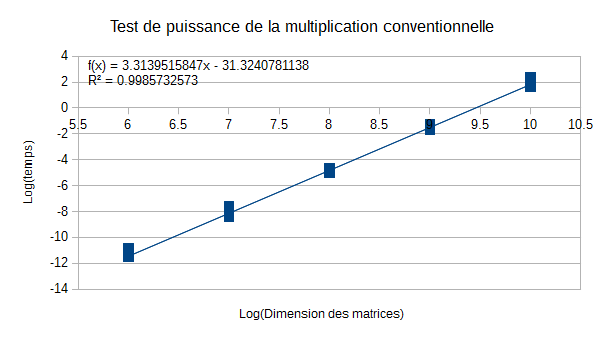
\includegraphics{Image/PuissanceConventionnelle.png}
\end{figure}

\begin{figure}[H]
\centering
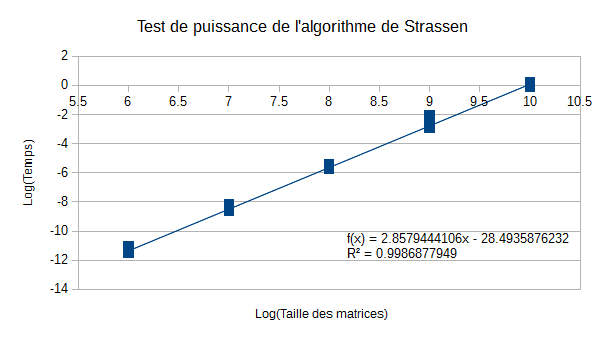
\includegraphics{Image/PuissanceStrassen.png}
\end{figure}

\begin{figure}[H]
\centering
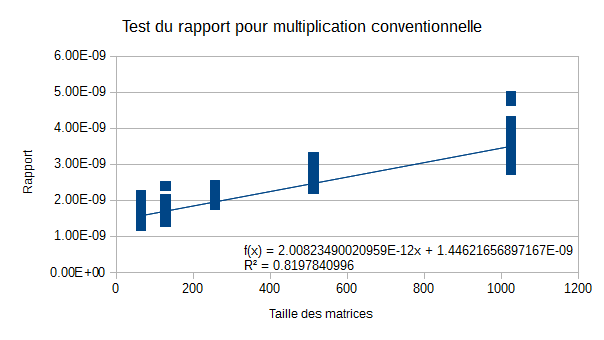
\includegraphics{Image/RapportConventionnelle.png}
\end{figure}

\begin{figure}[H]
\centering
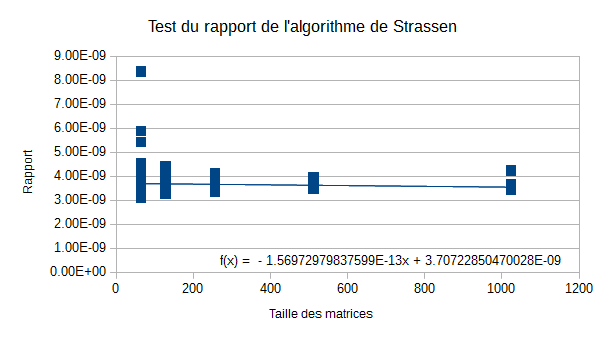
\includegraphics{Image/RapportStrassen.png}
\end{figure}

\begin{figure}[H]
\centering
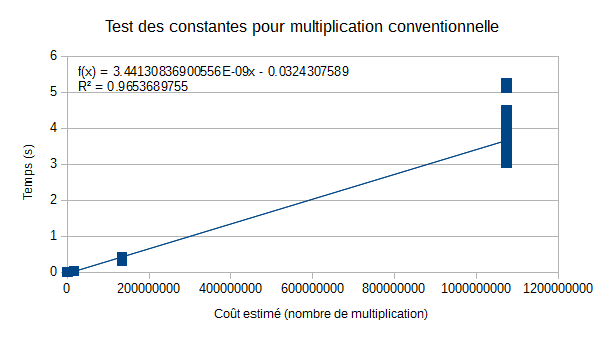
\includegraphics{Image/ConstantesConventionnelle.png}
\end{figure}

\begin{figure}[H]
\centering
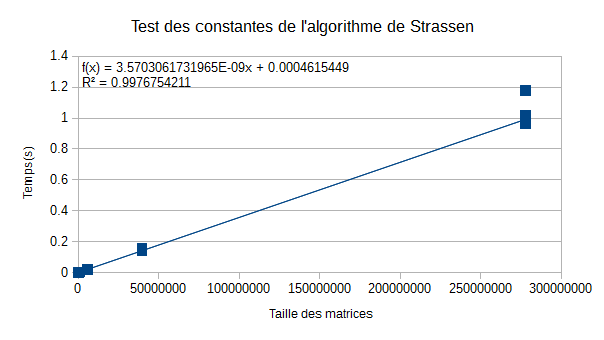
\includegraphics{Image/ConstantesStrassen.png}
\end{figure}

\section{Analyse et discussion}

\section{Conclusion}

\section{Bibliographie}
%----------------------------------------------------------------------------------------
\end{document}
\grid
